% =====================================================================
% 5. Area 2 in code: transfer from the ECG-GPT and zero-shot CLIP
%    (T13, T24: shared tasks, OF + MM)
% =====================================================================
\section{Area 2: learning strategies in code}\label{sec:strategies-code}

\subsection{Transfer from the ECG-GPT}

The pre-trained model is the generator of area 3 selected by the rule of that block (lowest validation
bits per sample), fixed before any transfer run: the ECG-GPT with one token per microvolt. Its summary
log hands over the model arguments, the checkpoints of the three seeds and the tokenizer; the transfer
run with seed $s$ loads the generator pre-trained with seed $s$, so the three seeds are three independent
pre-training + transfer pairs. Listing~\ref{lst:transfer} shows the classifier used by the three
strategies.

\lstinputlisting[firstnumber=185,caption={Generator backbone + new head (\texttt{src/transfer.py}, lines
185--212).},label={lst:transfer}]{common/code/transfer_classifier.py}

\begin{itemize}[leftmargin=1.2em,itemsep=1pt]
  \item \textbf{Loading.} The checkpoint is a \texttt{state\_dict}; it is loaded into a freshly built
        generator and the next-token head is discarded. \texttt{record\_features} averages the outputs of
        the final LayerNorm over the four windows of 250 samples that cover a record.
  \item \textbf{Freezing.} The linear probe sets \texttt{requires\_grad=False} on the backbone, and
        \texttt{train()} is overridden so that the backbone stays in evaluation mode even when the loop
        calls \texttt{model.train()}: its dropout is off and a record always gives the same vector, as a
        fixed feature extractor should.
  \item \textbf{A faster probe.} Because the frozen vectors never change, they are computed once per
        checkpoint and the head (\texttt{FeatureHead}) is trained on them; a test checks that this gives
        exactly the output of the frozen full model. A probe epoch takes
        \transferEpochTimeMedianProbeFOneZeroZero{}\,s against \transferEpochTimeMedianFinetuneFOneZeroZero{}\,s
        for fine-tuning with all the labels.
  \item \textbf{Learning rates.} $10^{-3}$ for the head and for training from scratch; $10^{-4}$ for
        fine-tuning, as in the optional fine-tuning cell of the course notebook \cite{course_nb_transfer}.
        Two ablations (fine-tuning at $10^{-3}$, scratch at $10^{-4}$) separate the effect of the
        pre-trained weights from that of the rate.
  \item \textbf{Memory.} One record is four windows of 250 tokens; the activations kept for
        backpropagation of 32 records already take about a gigabyte (measured on the CPU before the runs),
        so the transfer experiments use batches of 32 records instead of 64 on the 4\,GB GPU, the same for
        every configuration.
  \item \textbf{10\,\% of the labels, drawn by patient.} Training patients are shuffled with the run's
        seed and taken with all their records until 10\,\% of the training records is reached; the subset
        is the same for the three strategies of a seed (paired comparison) and its class counts are logged.
\end{itemize}

% Shared float (common/make_floats.py). Figure: figures/transfer_curves.pdf
\begin{figure}[htbp]
\centering
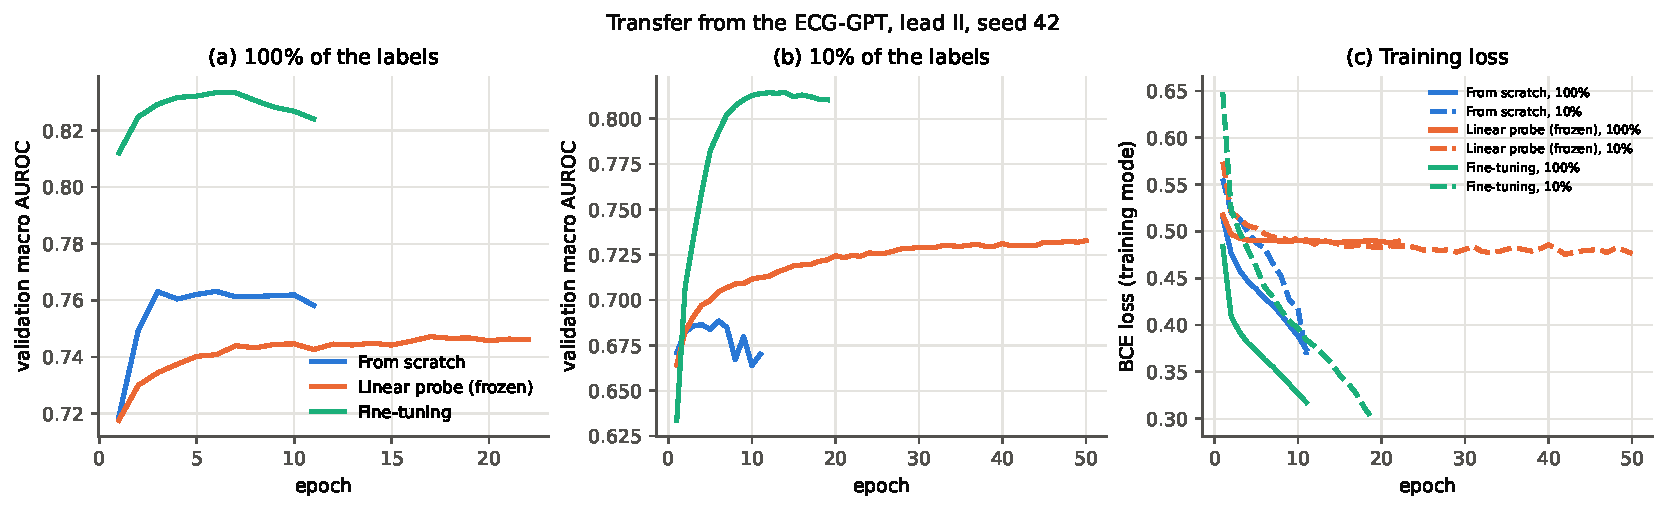
\includegraphics[width=\textwidth,height=0.42\textheight,keepaspectratio]{figures/transfer_curves.pdf}
\caption[Transfer from the ECG-GPT: learning curves]{Transfer from the ECG-GPT, lead II, seed 42: validation macro AUROC with (a) 100\,\% and (b) 10\,\% of the training labels, and (c) training loss of the three strategies.}
\label{fig:transfer_curves}
\end{figure}


The curves (Figure~\ref{fig:transfer_curves}) show what the numbers in the PRDL-DL report summarise:
fine-tuning starts high and peaks within a few epochs, training from scratch reaches its best epoch early (on average
\intval{\transferBestEpochMeanScratchFOneZeroZero} with all labels) and then overfits, and the probe with 10\,\% of the labels was still rising slowly near the 50-epoch limit (best
epoch \intval{\transferBestEpochMeanProbeFOneZero} on average): it was limited by the budget.

\subsection{Zero-shot with CLIP}

\begin{itemize}[leftmargin=1.2em,itemsep=1pt]
  \item \textbf{Model.} CLIP ViT-B/32 with OpenAI's weights, the model of the course notebook
        \cite{course_nb_clip}, loaded with \texttt{open\_clip}. The first run warned that open\_clip's plain
        \texttt{ViT-B-32} uses GELU while these weights were trained with QuickGELU, so the model is loaded
        as \texttt{ViT-B-32-quickgelu}. Nothing is trained or tuned.
  \item \textbf{Where zero-shot should work.} CIFAR-100 test images with the notebook's prompt and with the
        bare label; top-1 and top-5 accuracy with a bootstrap interval over images.
  \item \textbf{ECG as images.} Lead II of every validation and test record drawn as a $224\times224$
        image (two rows of 5\,s on a light grid, fixed scale), the size CLIP expects, so its preprocessing
        does not crop. One fixed sentence per superclass; class scores are the softmax over the five
        sentences of the scaled cosine similarity, as in the notebook. A modality check compares
        ``an electrocardiogram'' with five unrelated sentences.
  \item \textbf{A device bug} stopped the first run: image embeddings were moved to the CPU and text
        embeddings stayed on the GPU (documented in Mar\'ia's MLLB report, Sheet C3; error B10 of the AI log).
\end{itemize}

% Shared float (common/make_floats.py). Figure: figures/zeroshot_ptbxl.pdf
\begin{figure}[htbp]
\centering
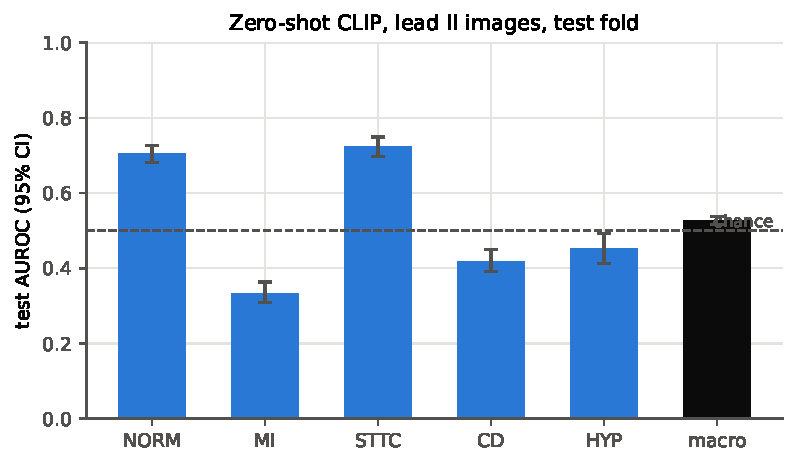
\includegraphics[width=\textwidth,height=0.42\textheight,keepaspectratio]{figures/zeroshot_ptbxl.pdf}
\caption[Zero-shot CLIP on PTB-XL]{Zero-shot CLIP on the test fold: AUROC per superclass and macro AUROC with 95\,\% patient-bootstrap intervals; dashed line: chance.}
\label{fig:zeroshot_ptbxl}
\end{figure}


\subsection{Twelve leads against lead II}

Every model class accepts \texttt{n\_leads=1}. The final model of each family was trained again on lead
II with everything else copied from its 12-lead final runs, as \texttt{--final} runs named
\texttt{onelead\_<family>\_...}, so they never mix with the 12-lead runs that each block's summary reads.
Results are in Table~\ref{tab:comparison_final}.
